%!TEX root=../document.tex

\section{Plattform}

Um eine Anwendung zu Entwickeln, welche es erlaubt, Daten zu synchronisieren und eine Offline-Verfügbarkeit mittels einer lokalen Client-Datenbank zu Verfügung zu stellen, gibt es einige unterschiedliche Ansätze.
\\\\
Wie bereits im Unterricht besprochen bietet diff-sync eine einfache Möglichkeit mittels Node.js Daten zu synchronisieren. Dieses Verfahren verwendet die Differential Synchronization Methode. \cite{nodejssync} Weiters gibt es unzählige Cloud Plattformen die solche Komplettlösungen anbieten, unter anderem Googles Firebase. Diese erlaubt es einfach, eine App zu Entwickeln, welche die Daten mit einer Firebase Datenbank zwischen Clients synchronisiert. \cite{firebase}
\\\\
Schlussendlich wurde Couchbase als Plattform zur Umsetzung dieser Übung gewählt, da es mittels Sync Gateway und Couchbase Lite die umfangreichste Plattform ist und die meisten Funktion bietet. Ebenso unterstützt Couchbase sehr viele unterschiedliche Systeme und Programmiersprachen. Unter anderem auch C\# mit UWP, wobei die mit der UWP und .Net Plattform entwickelte Anwendung mittels Xamarin auch auf Android und IOS laufen können. Da bereits einiges an Erfahrung mittels der Laborübung mit der UWP Plattform gesammelt worden ist, wurde für diese Aufgabe ebenfalls auf diese Plattform gesetzt. \cite{couchbasemobile}

\subsection{Couchbase}

Zur Umsetzung solch einer Anwendung mittels Couchbase werden drei Komponenten benötigt.

\begin{itemize}
	\item \textbf{Couchbase Server}: Ein NoSQL Server, welcher zentral alle Daten verwaltet und die Schnittstelle zum Sync Gateway bietet.
	\item \textbf{Sync Gateway}: Dies stellt die Schnittstelle zwischen den Server und den Clients dar. Sync Gateway bietet eine REST-Schnittstelle auf den Server zur Synchronisierung der Datensätze zugreift.
	\item \textbf{Couchbase Lite}: Stellt die Client Datenbank zu Verfügung. Kann offline verwendet werden und sobald eine Verbindung hergestellt werden kann, werden die Datensätze mittels Sync Gateway synchronisiert.
\end{itemize}

Einer der großen Vorteile dieser Plattform ist, dass der Client selber nie mit dem Server im Hintergrund kommuniziert bzw. diese Kommunikation umgesetzt werden muss. Die App selber greift nur auf die lokale Datenbank zu und nur diese Zugriffe müssen implementiert werden, die Synchronisierung übernimmt Sync Gateway und das Abspeichern der Couchbase Server. Außerdem kümmert sich Sync Gateway um die Versionierung der Dokumente sowie um das Lösen von Konflikten bei Dokumenten. \cite{couchbaseapp}


\begin{figure}[H]
	\centering
	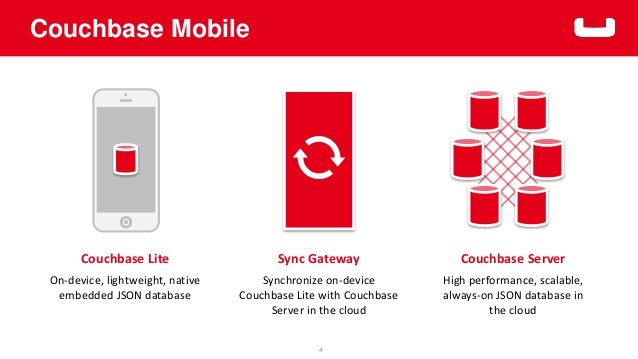
\includegraphics[width=0.95\linewidth]{img/building-net-apps-using-couchbase-lite-4-638}
	\caption{Umsetzung mittels Couchbase}
	\label{fig:building-net-apps-using-couchbase-lite-4-638}
\end{figure}


\section{Umsetzung}

Zum Umsetzen dieser Übung wurde auf den Server mit der IP-Adresse 37.252.185.24 ein Couchbase Server sowie Sync Gateway installiert. Mittels Visual Studio und C\# wurde ein UWP-App entwickelt, welche Couchbase Lite als lokale Datenbank verwendet und diese mit den Couchbase Server synchronisiert.

\subsection{Couchbase Server}

Zunächst wurde ein Couchbase Enterprise Server auf einen Server aufgesetzt, verwendet wurde die Version 5.1. Die Enterprise Edition darf kostenlos zur Entwicklung und Testen verwendet werden, erst beim normalen Betrieb muss eine Lizenz erworben werden.
\\\\
Der Server mit der Datenbank ist unter der IP-Adresse 37.252.185.24 und dem Port 8091 erreichbar. Beim Aufsetzen wurde ein neuer Cluster erstellt und die RAM Zuweisung wurde verringert, ansonsten wurden alle Einstellung bei den default Werten belassen.
\\\\
Über diese Adresse kann nun auf das Admin Dashboard des Couchbase Servers zugegriffen werden. Über dieses wurde ein Benutzer \textit{UserEin} erstellt, welche volle Zugriffsrechte auf den Bucket \textit{einkaufsliste} hat. \cite{couchbaseintro}

\subsection{Sync Gateway}

Wie auch der Couchbase Server wurde nun Sync Gateway auf dem Server installiert. Verwendet wurde die Version 2.0, diese kann nur in Kombination mit den Couchbase Server ab Version 5.0 verwendet werden. Auch hier muss kaum etwas konfiguriert werden, nur beim erstmaligem Starten des Services muss eine Konfigurationsdatei angegeben werden, diese sieht wie folgt aus:
\\\\
\begin{minted}{json}
	{
		"log": ["*"],
		"databases": {
			"db": {
				"server": "http://localhost:8091",
				"bucket": "einkaufsliste",
				"username": "UserEin",
				"password": "Einkaufsliste",
				"users": { "UserEin": { "disabled": false, "admin_channels": ["*"], "password": "Einkaufsliste" } },
				"sync": `function(doc) {
					channel("liste");
				}`
			}
		}
	}
	
\end{minted}

Diese JSON gibt den Namen der Datenbank an \textit{db}, weiters muss der Couchbase Server angegeben werden, dieser ist lokal mit dem Port 8091 aufrufbar. Der am Server erstellte Bucket mit dem Namen \textit{einkaufsliste} muss auch in der Konfiguration angegeben werden. Weiters muss der Benutzer sowie sein Passwort angegeben werden, sodass der Service mit dem Server kommunizieren kann. Abschließend gibt eine \textit{sync} Funktion an, welche Dokumente synchronisiert werden sollen. Hierbei kann mittels Tags gearbeitet werden, sodass ein Client nur bestimmte Dokumente synchronisiert, in diesem Fall wurden alle Dokumente dem Channel \textit{liste} hinzugefügt. \cite{couchbasechannel}
\\\\
Ob alles richtig funktioniert hat, kann einerseits anhand der Meldung in der Konsole überprüft werden, anderseits muss die Adresse mit dem Port 4984, bei einer erfolgreichem Konfiguration, folgendes zurückliefern. 

\begin{minted}{JSON}
	{"couchdb":"Welcome","vendor":{"name":"Couchbase Sync Gateway","version":"2.0"},"version":"Couchbase Sync Gateway/2.0.0(832;2d8a6c0)"}
\end{minted}

Wichtig zu beachten ist, sobald Sync Gateway aufgesetzt worden ist, sollte das Admin Dashboard des Couchbase Servers nicht mehr zum Verwalten der Dokumente verwendet werden, dies könnte nämlich zu Problemen bei der Synchronisierung zu den Clients führen. Sync Gateway bietet eine REST-Schnittstelle, über welche alle Dokumente im Bucket verwaltet werden können. \cite{syncgateway} 

\subsection{Couchbase Lite}

Wie bereits oben erwähnt wurde bei dieser Übung auf die UWP Plattform zurückgegriffen, da bei der letzten Übung bereits einiges an Erfahrung gesammelt worden ist und die Entwicklung sowie das Testen einfacher und schneller ist, da die Anwendung auch lokal getesten werden kann und nicht in einem Emulator oder auf einem Smartphone getesten werden muss.
\\\\
Um Couchbase Lite dem Projekt hinzuzufügen, muss das NuGet Package \textit{Couchbase.Lite.Enterprise} installiert werden, dies kann über den NuGet Package Manager in Visual Studio gemacht werden.
\\\\
Die App bietet eine einfache Benutzeroberfläche, welche alle Gegenstände in einer Liste darstellt, diese können bearbeitet oder gelöscht werden. Über zwei Eingabefelder am unteren Rand, können neue Items zur Liste hinzugefügt werden. Dafür muss nach der Eingabe der Werte auf den \textit{Hinzufügen} Button geklickt werden. Das Item wird sofort in der Liste angezeigt und nach kurzer Zeit, wenn möglich, auch synchronisiert und bei anderen Benutzern angezeigt.
\\\\
Um einen Eintrag zu bearbeiten, muss dieser aus der Liste ausgewählt werden. Über den \textins{Bearbeiten} Button können nun die Werte geändert werden. Mittels dem \textit{Speichern} Button können diese Änderungen gespeichert werden. Auch bei Änderungen wird der Eintrag sofort am Client angezeigt und nach kurzer Zeit bei anderen Benutzern.
\\\\
Um Einträge zu löschen, kann ganz einfach der \textit{X} Button bei dem entsprechendem Eintrag getätigt werden. Diese Änderung wird ebenfalls sofort synchronisiert.

\begin{figure}[H]
	\centering
	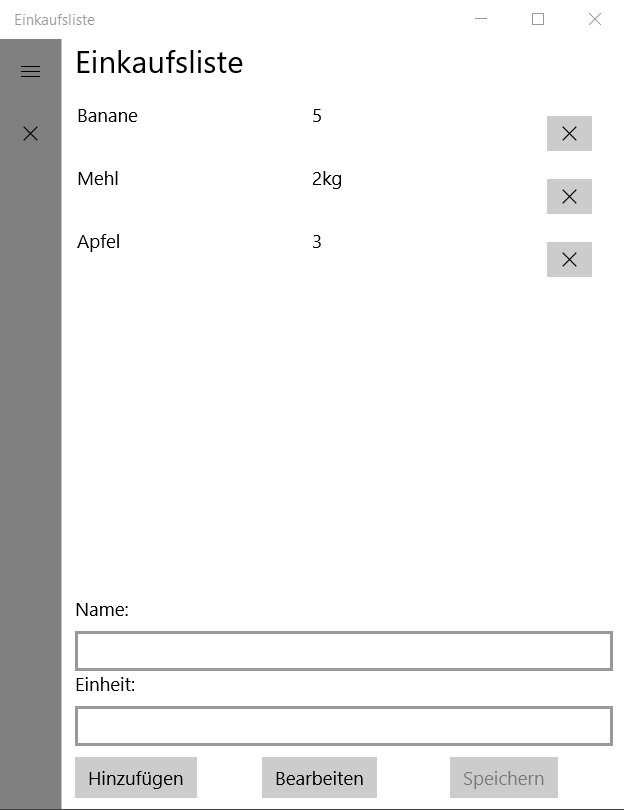
\includegraphics[width=0.7\linewidth]{img/screenshot001}
	\caption{Benutzeroberfläche der Einkaufsliste}
	\label{fig:screenshot001}
\end{figure}

\subsubsection{Benutzeroberfläche}

Zur Darstellung der Einträge wurde eine ListView verwendet, diese stellt alle Objekte dar, welche der ObservableCollection hinzugefügt werden. Um dies Umzusetzen, wurde ein Objekt namens \textit{Item} erstellt, dieses beinhaltet alle wichtigen Informationen und wird für die Darstellung in der Liste verwendet. \cite{listview}

\begin{minted}{xml}
<ListView x:Name="MyListView" Grid.Row="1" Grid.Column="0" ItemsSource="{x:Bind ViewModel.Items}" SelectionChanged="ListView_OnSelectionChanged" HorizontalAlignment="Stretch" HorizontalContentAlignment="Stretch">
	<ListView.ItemTemplate>
		<DataTemplate x:DataType="Einkaufsliste:Item">
		<Grid>
			<TextBlock Grid.Column="0" Text="{x:Bind Name}" Height="50" VerticalAlignment="Center" />
			<TextBlock Grid.Column="1" Text="{x:Bind Value}" x:Phase="1" Height="50" VerticalAlignment="Center"/>
			<Button Grid.Column="2" x:Name="delete" FontFamily="Segoe MDL2 Assets" DataContext="{x:Bind ID}" Content="&#xE10A;" Click="Button_Click_Delete" />	
		</Grid>
		</DataTemplate>
	</ListView.ItemTemplate>
</ListView>
\end{minted}

Alle Informationen, welche angezeigt werden sollen, werden in den Objekt namens \textit{Item} gespeichert. Dieses Objekt beinhaltet den Namen sowie die Menge. Zur eindeutigen Identifikation übernimmt das Objekt noch die ID des Couchbase Documents.

\begin{minted}{csharp}
public class Item
{
	public string ID { get; set; }
	public string Name { get; set; }
	public string Value { get; set; }
}
\end{minted}

Wobei die Klasse ItemViewModel sich um das Verwalten der Collection von Items kümmert. In dieser Klasse werden beim Start des Programmes alle Objekte ausgelesen, sowie bei der Synchronisierung die Objekteinformationen aktualisiert, sodass die neuen Informationen angezeigt werden. \cite{listview}

\subsubsection{Lokale Datenbank}

In der App Klasse wurde die Methode \textit{StartDBConnection} erstellt, diese baut eine Verbindung zur lokalen Datenbank auf und falls möglich, wird die Synchronisierung mit dem Couchbase Server gestartet. Diese Methode wird beim Start der App aufgerufen und aktiviert als erstes den UWP Support und erstellt bzw. verbindet sich zu der Datenbank \textit{einkaufsliste}.

\begin{minted}{csharp}
Couchbase.Lite.Support.UWP.Activate();
this.database = new Database("einkaufsliste");
\end{minted}

Nun muss die Konfiguration für die Replikation erstellt werden und hierfür muss ein Endpoint bestimmt werden. Als Replicator Type wurde Push und Pull gewählt. Weiters muss der Channel angegeben werden, welcher in der Sync Gateway Konfigurationsdatei festgelegt worden ist. Abschließend muss noch die Authentifikation konfiguriert werden, nun kann die Replikation gestartet werden. \cite{couchbasegettingstarted}

\begin{minted}{csharp}
var targetEndpoint = new URLEndpoint(new Uri("ws://37.252.185.24:4984/db"));
var replConfig = new ReplicatorConfiguration(this.database, targetEndpoint)
{
	ReplicatorType = ReplicatorType.PushAndPull
};
replConfig.Channels = new List<String>();
replConfig.Channels.Add("liste");
replConfig.Continuous = true;

replConfig.Authenticator = new BasicAuthenticator("UserEin", "Einkaufsliste");

var replicator = new Replicator(replConfig);
replicator.Start(); 
\end{minted}

Nun kann in der MainPage die Verbindung zur lokalen Datenbank verwendet werden, um CRUD Operationen durchzuführen.

\subsubsection{Synchronisierung}

Nun wird die lokale Datenbank mit dem Server synchronisiert, um auf die Änderungen der lokalen Datenbank zu reagieren, welche durch die Synchronisierung durchgeführt werden, muss ein Change Listner auf die Datenbank gelegt werden. Dieser wird immer ausgelöst, wenn eine Änderung an der Datenbank durchgeführt wird. Dieser Listner ruft die Methode \textit{UpdateAll} auf, diese liest alle Dokumente aus der Datenbank aus und aktualisiert die \textit{Items} Objekte für die Darstellung.

\begin{minted}{csharp}
this.param.App.database.AddChangeListener((sender, args) =>
{
	this.ViewModel.UpdateAll();
});
\end{minted}

In dieser Methode wird mittels einem QueryBuilder eine Query erstellt, welche alle Dokumente aus der Datenbank ausliest. Die Ergebnisse können zu einer Liste gecastet werden. Mittels dem enthaltenem Dictionary kann auf die Werte der Dokumente zugegriffen werden. \cite{couchbasegettingstarted}

\begin{minted}{csharp}
using (var query = QueryBuilder.Select(SelectResult.All())
.From(DataSource.Database(this.param.App.database)))
{
	var result = query.Execute();
	var res = result.ToArray();
	
	var documents = new List<string>();
	foreach (var i in res)
	{
		foreach (var item in Items)
		{
			item.Name = i.GetDictionary(0).GetString("name");
			item.Value = i.GetDictionary(0).GetString("value");
			documents.Add(item.ID);
			found = true;
			break;
		}
	}
}
\end{minted}

\subsubsection{Löschen eines Eintrages}

In der ListView hat jeder Eintrag einen Löschen Button, dieser hat im DataContext die ID des Dokumentes gespeichert. Bei einem Click Event wird die Methode \textit{Button\_Click\_Delete} aufgerufen, diese castet den Sender zu einem Button um und holt sich aus dem DataContext die ID. Mittels dieser ID kann aus der Datenbank das Dokument gelöscht werden. \cite{uwpbutton}

\begin{minted}{csharp}
private void Button_Click_Delete(object sender, RoutedEventArgs e)
{
	Windows.UI.Xaml.Controls.Button button = (Windows.UI.Xaml.Controls.Button)sender;
	Document doc = this.param.App.database.GetDocument((string) button.DataContext);
	this.param.App.database.Delete(doc);
	
}
\end{minted}

\subsubsection{Hinzufügen eines Eintrages}

Wird der Button \textit{Hinzufügen} geklickt, werden die Eingaben in die Felder überprüft, falls diese leer sind, wird der Benutzer mittels einem PopUp informiert, dass diese nicht leer sein dürfen. Ist dies nicht der Fall, wird ein neues Dokument erstellt. Hierfür wird ein MutableDocument erstellt, dieses bekommt automatisch eine ID zugewiesen, das Dokument wird anschließend in die Datenbank gespeichert. \cite{couchbasegettingstarted}

\begin{minted}{csharp}
public void AddItem(string name, String value)
{
	using (var mutableDoc = new MutableDocument())
	{
		mutableDoc.SetString("name", name).SetString("value", value).SetString("ID", mutableDoc.Id);
		this.database.Save(mutableDoc);
	}
}
\end{minted}

\subsubsection{Update eines Eintrages}

Wenn der Benutzer einen Eintrag bearbeitet, werden die Werte in die Eingabefelder geschrieben, diese kann der Benutzer bearbeiten. Klickt der Benutzer anschließend auf den \textit{Speichern} Button, wird das Dokument mit der ID aus der Datenbank ausgelesen, die Werte aktualisiert und wieder in die Datenbank abgespeichert. \cite{couchbasegettingstarted}

\begin{minted}{csharp}
using (var doc = this.param.App.database.GetDocument(this.id))
using (var mutableDoc = doc.ToMutable())
{
	mutableDoc.SetString("name", this.name.Text);
	mutableDoc.SetString("value", this.value.Text);
	this.param.App.database.Save(mutableDoc);
}
\end{minted}